\chapter{実験と考察}
\thispagestyle{myheadings}

\section{はじめに}
本章では,提案システムを実装し,大学生の被験者に対してアンケート評価を行う.そして,各実験のアンケート評価の結果から考察について述べる.
アンケート評価にはSD法を使用した.提案システムに対しての心理的尺度を図り,リハビリに対するモチベーションへの影響を考察する.
\section{実験環境}
実験環境を以下に示す.

\begin{itemize}
 \item OS: Windows8.1
 \item CPU: 4.0GHz Intel Corei7-4790k
 \item GPU: 4GB NIVIDA Geforce GTX970
 \item Memory: 8G DDR3-1600×2
\end{itemize}

HMDには,Oculus VR社のOculusRiftDK2\cite{OculusRift}を使用した.開発環境はUnity\cite{Unity}を使用した.開発環境であるUnityで提供されている3D都市モデル空間アセット\cite{3D都市モデル}を仮想空間として使用する.使用キャラクタを図\ref{fig:chara}に示す.下肢リハビリ装置の動作周波数を約1.67 秒の1周期ごととし,CGキャラクタが0.64m進む設定とした.

\begin{figure}[tbp]
	\centering
			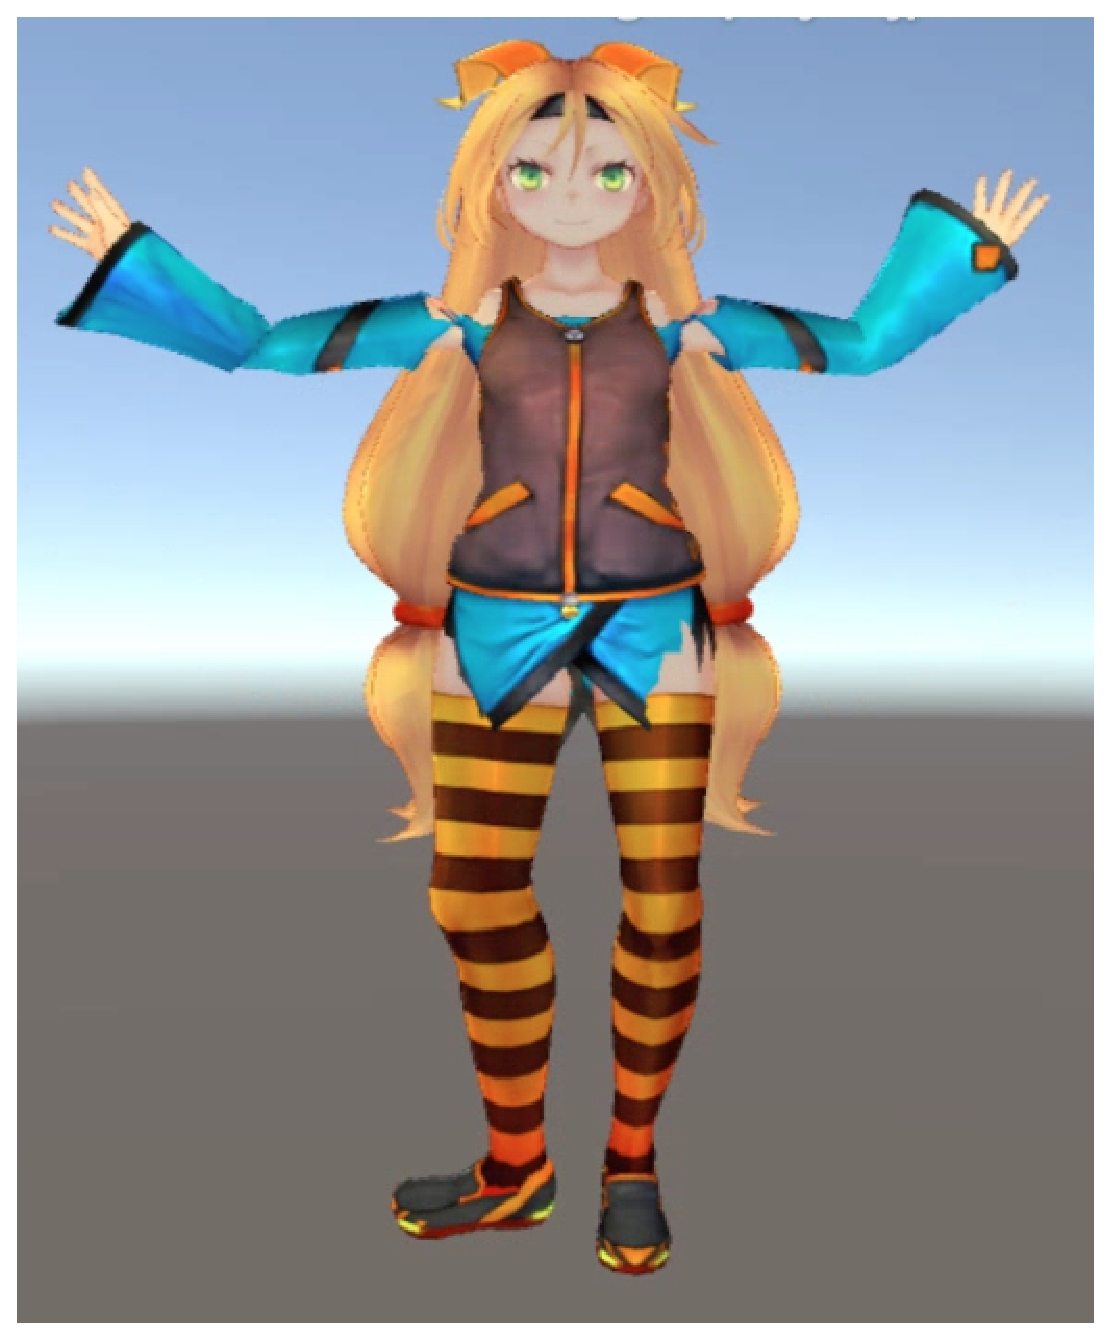
\includegraphics[width=0.5\textwidth]{chap3-figure/UntyChan.eps}
	\caption{使用キャラクタ\protect \footnotemark}
	\label{fig:chara}
\end{figure}
\footnotetext{Unity Technologies Japan/UCL}

\section{使用アンケート}
評価対象は,提案システムを使用した実験(実験1),ベッド型の下肢リハビリ装置のみを使用した実験(実験2),提案システムにおいて風景を変化させない実験(実験3),ベッド型の下肢リハビリ装置を動作させず,HMD の映像のみを視聴した実験(実験4) の4 種類を用意した.10 代から20 代の男性24 名を対象にSD 法の形容詞対と記述式の2種類のアンケートを用いた.使用したアンケートを図\ref{fig:ank1}--\ref{fig:ank4}に示す.実験の体験時間は3 分間である.実験の様子を図\ref{fig:jiken}示す.

\subsection{SD法とは}
SD法\cite{人間工学ガイド}は相反する形容詞対を多数用いて評価することにより,人が「どのように感じるか」といった心理的な印象を明らかにすることができる.今回の実験では,提案システムの絶対的な印象を評価するために,各実験6名ずつに分かれて実験を行った.

\subsection{実験の種類}
評価対象は,提案システムを使用した実験(実験1),ベッド型の下肢リハビリ装置のみを使用した実験(実験2),提案システムにおいて風景を変化させない実験(実験3),ベッド型の下肢リハビリ装置を動作させず,HMD の映像のみを視聴した実験(実験4) の4 種類を用意した.10代から20代の男性24名を対象にSD 法の形容詞対と記述式の2種類のアンケートを用いた.

\begin{figure}[tbp]
	\centering
		\fbox{
			\includegraphics[width=0.9\textwidth]{chap3-figure/a-0.eps}
			}
	\caption{アンケート1枚目}
	\label{fig:ank1}
\end{figure}

\begin{figure}[tbp]
	\centering
		\fbox{
			\includegraphics[width=0.9\textwidth]{chap3-figure/a-1.eps}
		}
	\caption{アンケート2枚目}
	\label{fig:ank2}
\end{figure}
\begin{figure}[tbp]
	\centering
	\fbox{
			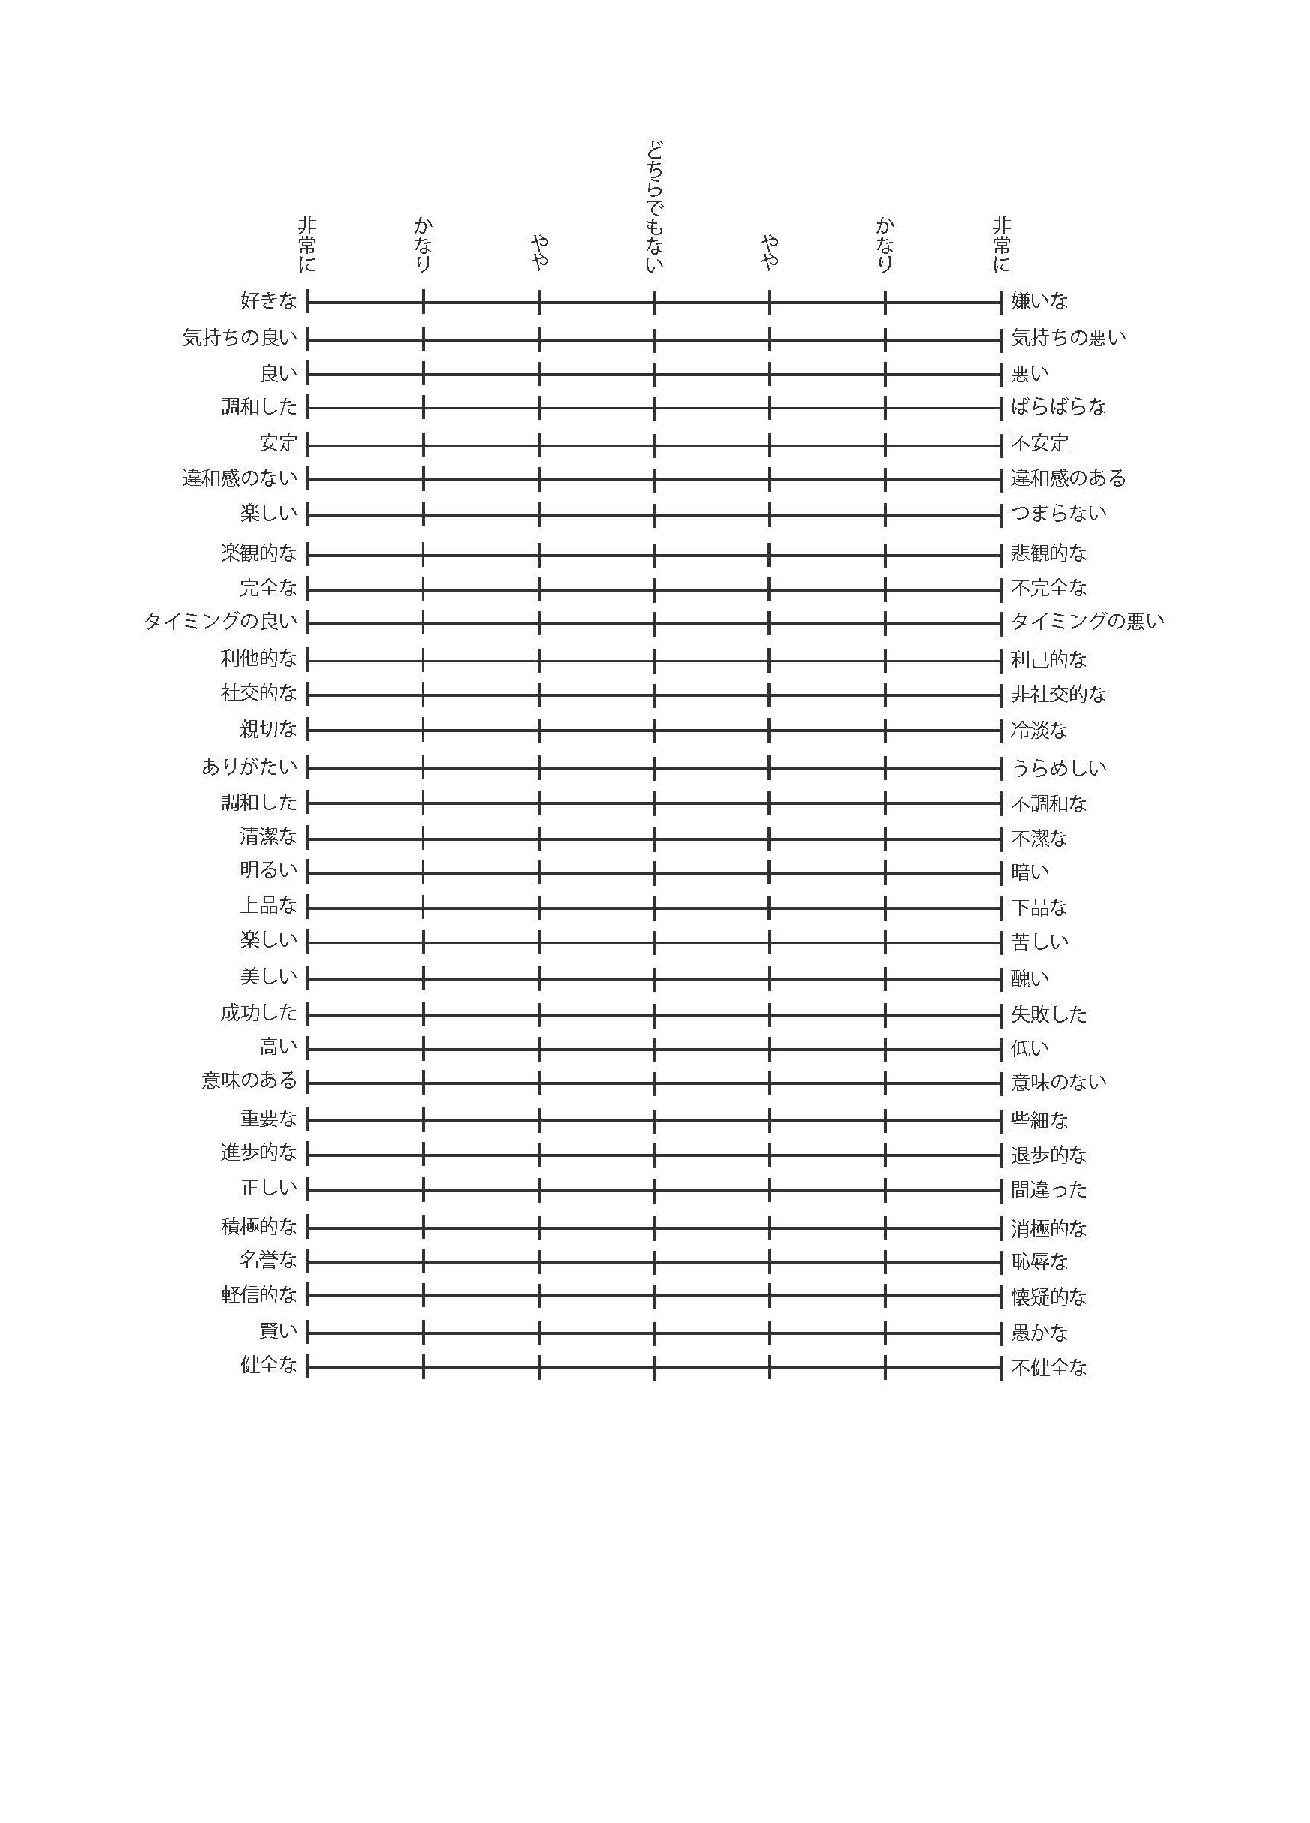
\includegraphics[width=0.9\textwidth]{chap3-figure/a-2.eps}
			}
	\caption{アンケート3枚目}
	\label{fig:ank3}
\end{figure}
\begin{figure}[tbp]
	\centering
	\fbox{
			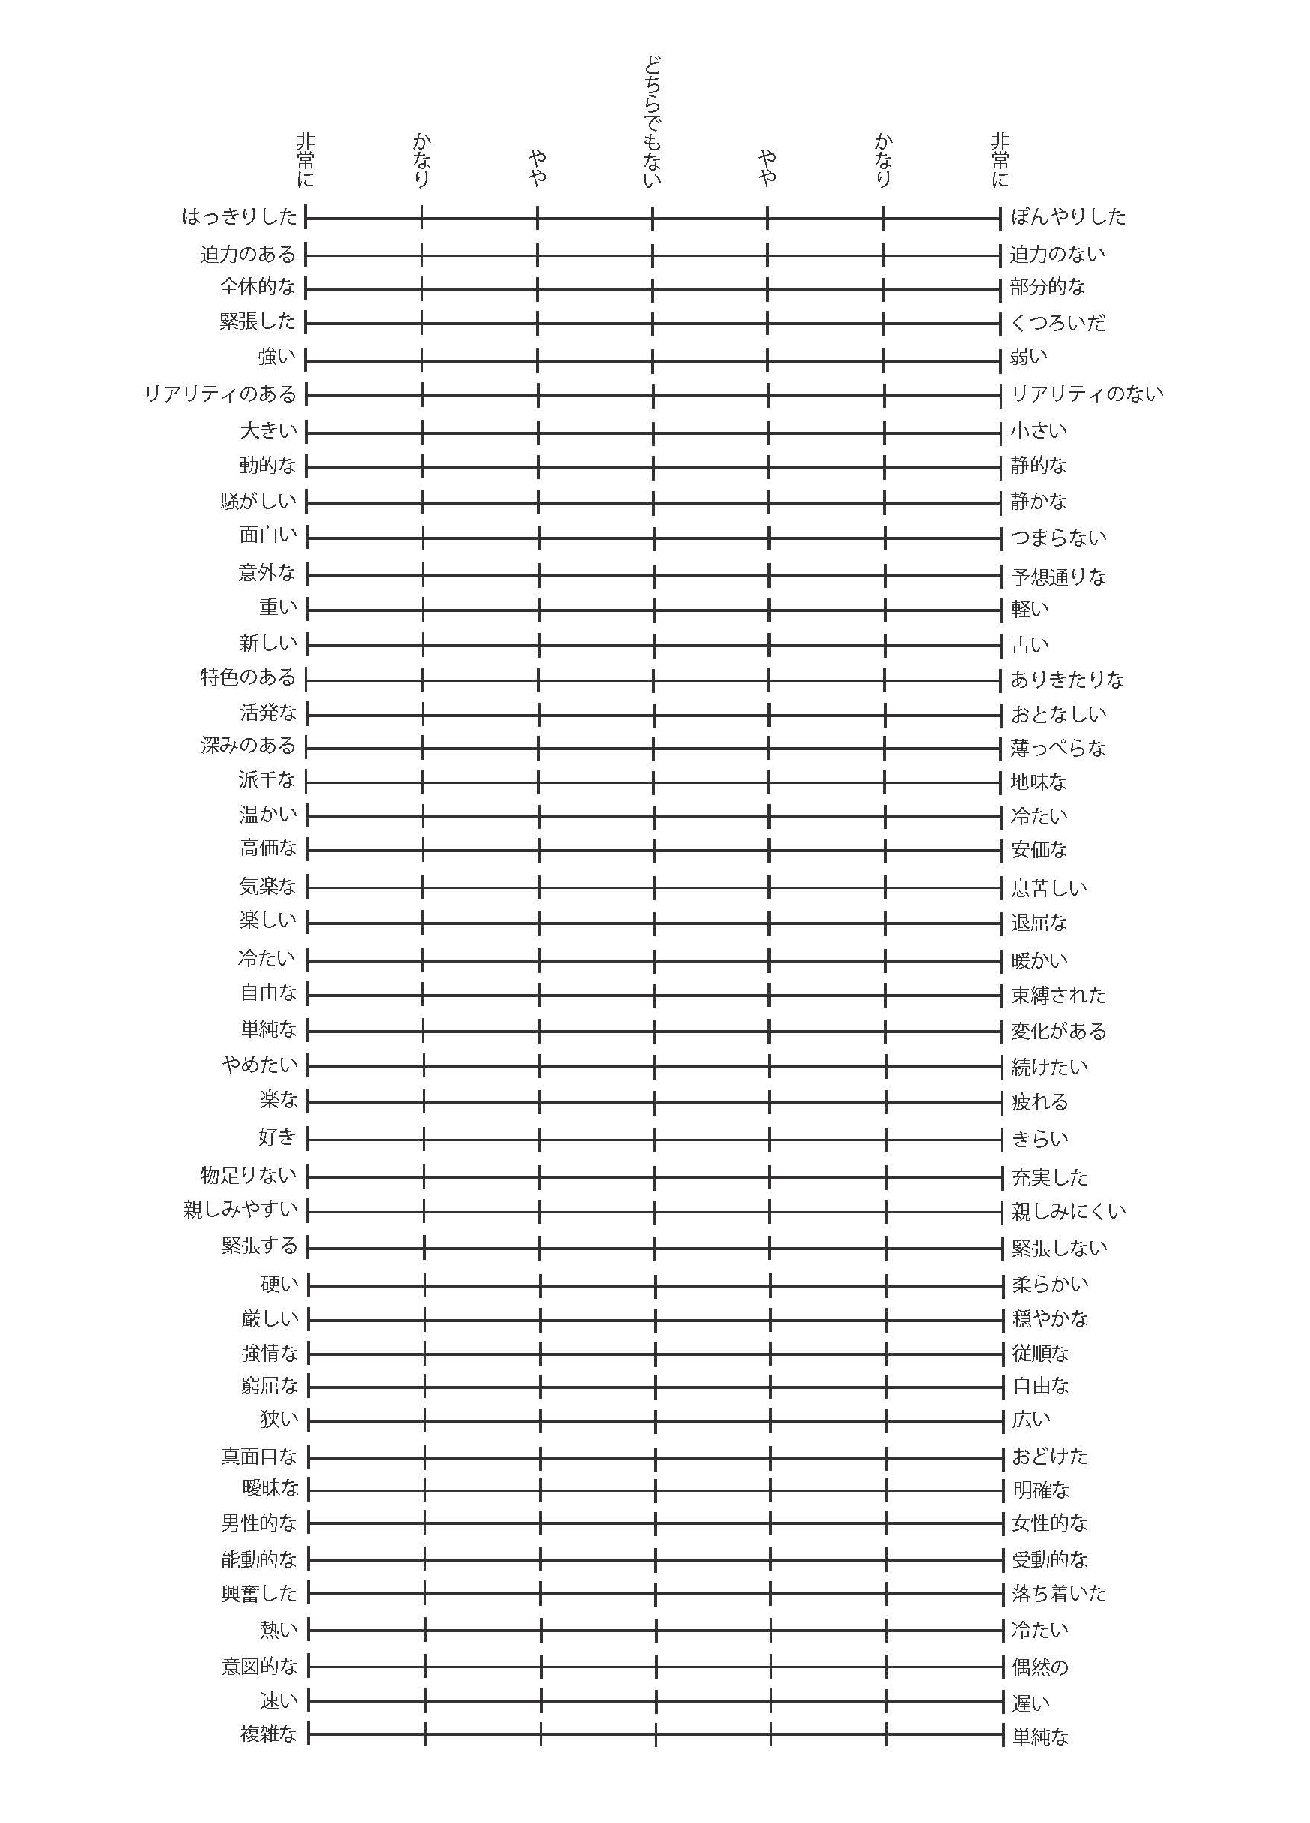
\includegraphics[width=0.9\textwidth]{chap3-figure/a-3.eps}
			}
	\caption{アンケート4枚目}
	\label{fig:ank4}
\end{figure}

\begin{figure}[tbp]
	\centering
			\includegraphics[width=0.8\textwidth]{chap3-figure/jiken.eps}
	\caption{実験風景}
	\label{fig:jiken}
\end{figure}

\begin{figure}[tbp]
	\centering
			\includegraphics[width=0.8\textwidth]{chap3-figure/ankert.eps}
	\caption{アンケート回答の様子}
	\label{fig:ankkai}
\end{figure}

\section{考察}
アンケートで得られた結果を基に考察を行う.アンケートの回答の様子を図\ref{fig:ankkai}に示す.また,自由記述の回答時間は3分間とした.

\subsection{SD法アンケート考察}
各実験およびアンケート評価の結果から考察について述べる.各実験の平均値\cite{average}を算出し,モチベーションに関わる形容詞対を抜粋し比較を行った.実験1と実験2で各形容詞対の尺度の平均値を比較し,セマンティック・プロフィール\cite{sd_zu}で図示することで提案システムによる印象の影響を調べた.

実験1と実験2を比較したアンケート結果を図\ref{fig:j-1-2}に示す.図\ref{fig:j-1-2}から実験1 と実験2を比較して,楽しい・面白い・新しい・遅い・健全な・好き,という印象が得られた.これらの結果から提案システムは好印象であることが考えられる.一方でネガティブな「遅い」という印象を解決することが今後の課題といえる.


実験1と実験3を比較したアンケート結果を図\ref{fig:j-1-3}に示す.図\ref{fig:j-1-3}から実験1 と実験3を比較して,楽しい・面白い・新しい・遅い・健全な・嫌いな,という印象が得られた.これらの結果から提案システムは好印象の面もあるが改善点もあると考えられる.一方でネガティブな「遅い」,「嫌い」という印象を解決することが今後の課題といえる.


実験1と実験4を比較したアンケート結果を図\ref{fig:j-1-4}に示す.図\ref{fig:j-1-4}から実験1 と実験4を比較して,楽しい・面白い・新しい・遅い・健全な・嫌いな,という印象が得られた.これらの結果から提案システムは好印象の面もあるが改善点もあると考えられる.一方でネガティブな「遅い」,「嫌い」という印象を解決することが今後の課題といえる.


以上の結果から,実験1の提案システムを使用した下肢リハビリがリハビに対するモチベーションの向上に繋がることが考えられる.
また,マン・ホイットニーのU検定\cite{U検定}を使用し各実験の形容詞対に有意差が見られた形容詞対を示す結果を示す.

実験1と実験2では形容詞対の有意差は確認できず,実験1と実験3では,実験1の条件のほうが「緊張する」と回答する傾向が得られた.また,実験3の条件のほうが「良い」「明るい」「迫力のある」「温かい」「熱い」と回答する傾向があった.実験1と実験4では,実験4の条件のほうが「全体的な」「能動的な」と回答する傾向が確認できた.
\begin{figure}[tbp]
	\centering
			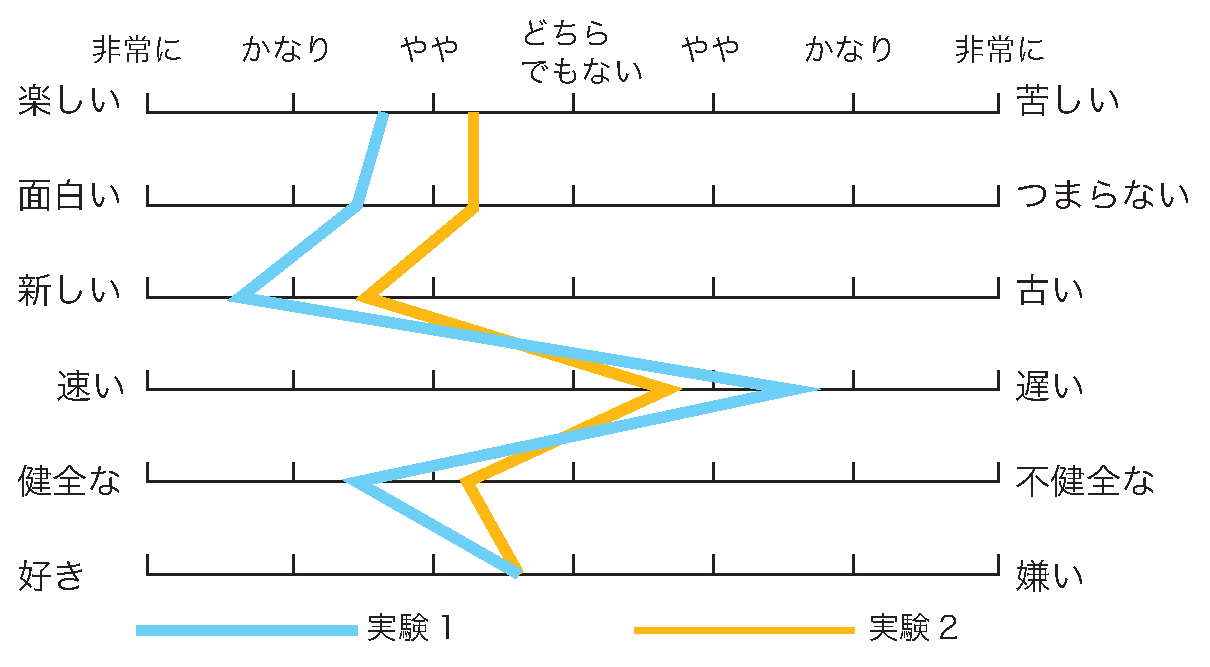
\includegraphics[width=0.9\textwidth]{chap3-figure/j-1-2.eps}
	\caption{実験1と実験2のセマンティック・プロフィール}
	\label{fig:j-1-2}
\end{figure}

\begin{figure}[tbp]
	\centering
			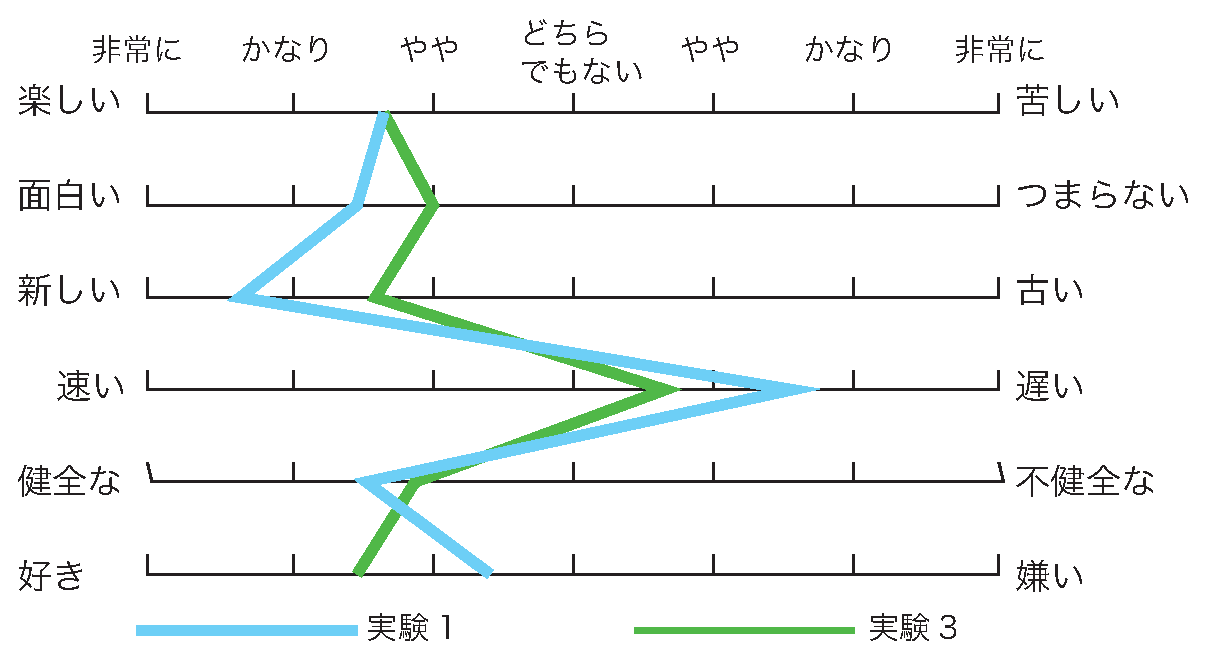
\includegraphics[width=0.9\textwidth]{chap3-figure/j1-3.eps}
	\caption{実験1と実験3のセマンティック・プロフィール}
	\label{fig:j-1-3}
\end{figure}
\begin{figure}[tbp]
	\centering
			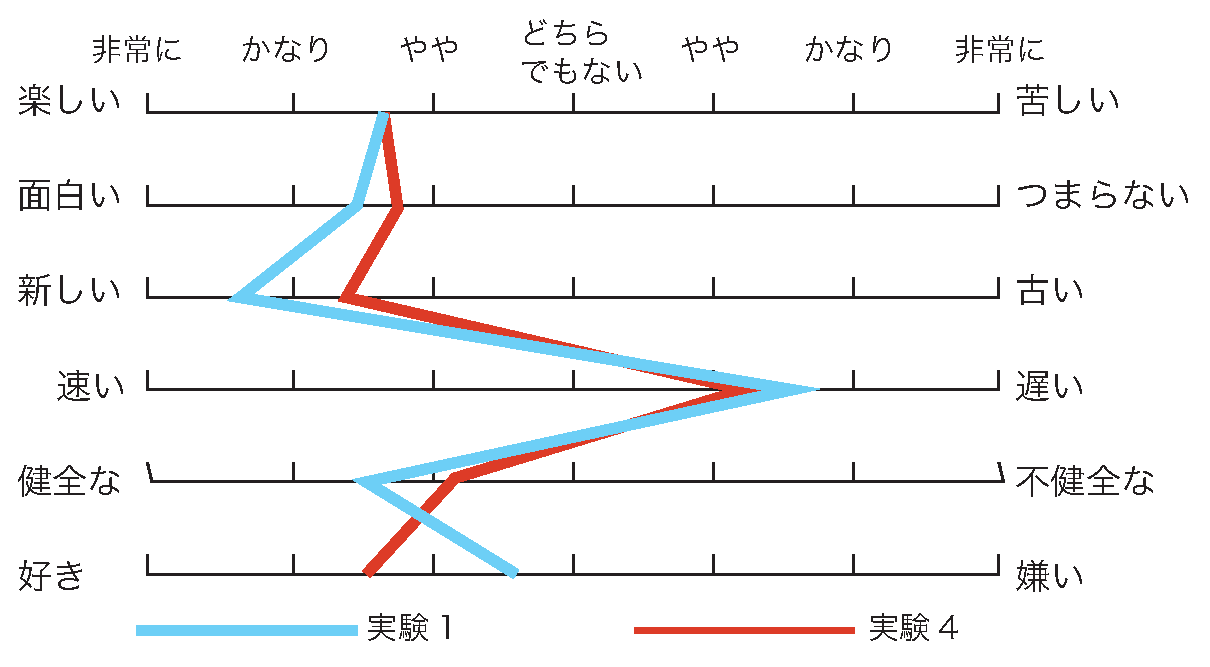
\includegraphics[width=0.9\textwidth]{chap3-figure/j1-4.eps}
	\caption{実験1と実験4のセマンティック・プロフィール}
	\label{fig:j-1-4}
\end{figure}

\subsection{自由記述アンケート考察}
自由記述アンケートを行った際の個人間の回答の主な頻出ワードを提示し,個人間の回答の傾向をつかむ.実験1の記述式アンケートの結果を図\ref{fig:j-1}に示す.図\ref{fig:j-1}から,実験1では「楽しい・面白い」や「面白い」といったリハビリに対してポジティブな意見が確認された.また,「歩いているようだ」や「足のトレーニングになりそう」といったリハビリに対するポジティブな意見も出された.

実験2の記述式アンケートの結果を図\ref{fig:j-2}に示す.図\ref{fig:j-2}から,実験2では「歩いている感じ」や「暇・他事ができそう」や「作動音がうるさい」といった意見が確認された.「作動作音がうるさい」といった意見から,被験者にヘッドフォンを着用し,生活音も出力するシステムへの変更も検討される.これにより臨場感が高まり,没入感の向上が期待できる.

実験3の記述式アンケートの結果を図\ref{fig:j-3}に示す.図\ref{fig:j-3}から,実験3では「楽しかった」や「景色が変わらないのは不自然」や「景色が綺麗」や「歩いているような」といった意見が確認された.結果から,被験者は下肢リハビリを行っているのにキャラクタの移動がないと違和感を感じる意見が確認された.

実験4の記述式アンケートの結果を図\ref{fig:j-4}に示す.図\ref{fig:j-4}から,実験4では「面白い」や「楽しい」や「ゆっくりとした」といった意見が確認された.結果から,歩行の感覚が長くゆっくりとしたといった,意見が出されたと考えられる.

\begin{figure}[!tbp]
	\centering
			\includegraphics[width=0.8\textwidth]{chap3-figure/j1.eps}
	\caption{実験1の自由記述}
	\label{fig:j-1}
\end{figure}
\begin{figure}[!tbp]
	\centering
			\includegraphics[height=0.7\textwidth]{chap3-figure/j2.eps}
	\caption{実験2の自由記述}
	\label{fig:j-2}
\end{figure}
\begin{figure}[!tbp]
	\centering
			\includegraphics[width=0.9\textwidth]{chap3-figure/j3.eps}
	\caption{実験3の自由記述}
	\label{fig:j-3}
\end{figure}
\begin{figure}[!tbp]
	\centering
			\includegraphics[width=0.9\textwidth]{chap3-figure/j4.eps}
	\caption{実験4の自由記述}
	\label{fig:j-4}
\end{figure}

\section{むすび}
本章では,提案システムの実装を行い,提案システムと他動歩行器具を被験者に対して使用したアンケート評価について述べた.そして,それぞれの実験に対しての考察を行った.

% Local Variables: 
% mode: japanese-LaTeX
% TeX-master: "root"
% End: 
